\documentclass{article}

% Use the official NeurIPS 2025 style file placed in this directory.
% IMPORTANT: For anonymous submission, DO NOT pass [preprint] or [final].
% Line numbers are added automatically during submission.
\usepackage{neurips_2025}

% Common packages (keep minimal and template-compliant)
\usepackage[utf8]{inputenc}
\usepackage[T1]{fontenc}
\usepackage{hyperref}
\usepackage{url}
\usepackage{booktabs}
\usepackage{amsfonts}
\usepackage{nicefrac}
\usepackage{microtype}
\usepackage{graphicx}
\usepackage{amsmath, amssymb}
\usepackage{enumitem}

\title{GrowNet: Learning-first, self-growing neural networks with slot-gated neurons}

% Anonymous by default; fill only for camera-ready
\author{Anonymous Authors}
\date{}

\begin{document}
\maketitle

\begin{abstract}
We introduce GrowNet, an online, locally learned architecture whose neurons contain independent slots with adaptive thresholds (T0+T2) and bounded reinforcement. GrowNet supports growth on out-of-distribution stimuli and relies on lateral buses for inhibition and modulation, without backpropagation. On few-shot image tasks, GrowNet aims to match baselines with substantially less data. We detail the mechanism and provide evidence across controlled benchmarks.
\end{abstract}

\section{Introduction}
\paragraph{Problem.} Modern deep learning relies on large IID datasets and offline training; continual, online learning with data-efficiency remains challenging.

\paragraph{Idea.} \textbf{GrowNet} is an event-driven architecture where each neuron contains multiple slot-like subunits with adaptive thresholds (T0 imprint + T2 homeostasis). Learning is local and bounded; capacity grows when stimuli fall outside covered regimes.

\paragraph{Contributions.} (i) A unified onInput/onOutput neuron contract enabling clean actuator boundaries; (ii) a hybrid T0+T2 threshold update rule that stabilizes spike rates near a target; (iii) a simple growth/pruning policy; (iv) cross-language reference implementations (Python/Java/C++/Mojo) and image I/O demos.

\section{Related Work}
We focus on minimal, positioning context. Detailed engineering references are placed in the appendix or cited repository. We compare to: spiking and event-based nets, few-shot/meta-learning baselines, and dynamic-capacity networks.

\section{Method}
\subsection{Neuron with Slots}
Each neuron holds a map of slots (weights). Each slot maintains a strength, adaptive threshold, spike-rate EMA, a first-seen flag, and a hit counter up to a saturation limit.

\subsection{Local Learning (bounded reinforcement)}
Strengths are updated with a bounded, non-linear rule scaled by a modulation factor and tempered by inhibition on the layer bus.

\subsection{Adaptive Thresholds (T0+T2)}
On first effective stimulus, T0 sets the threshold just below it. Subsequently, T2 homeostasis nudges the threshold by $\eta\,(\hat r - r^\star)$ where $\hat r$ is the slot's firing EMA.

\subsection{Network Dynamics}
Layers own a lateral bus (inhibition/modulation). Regions orchestrate a two-phase tick: Phase A injects inputs and allows local propagation; Phase B flushes inter-layer tracts once. Output neurons never propagate; instead they accumulate and finalize a frame via EMA.

\begin{figure}[t]
  \centering
  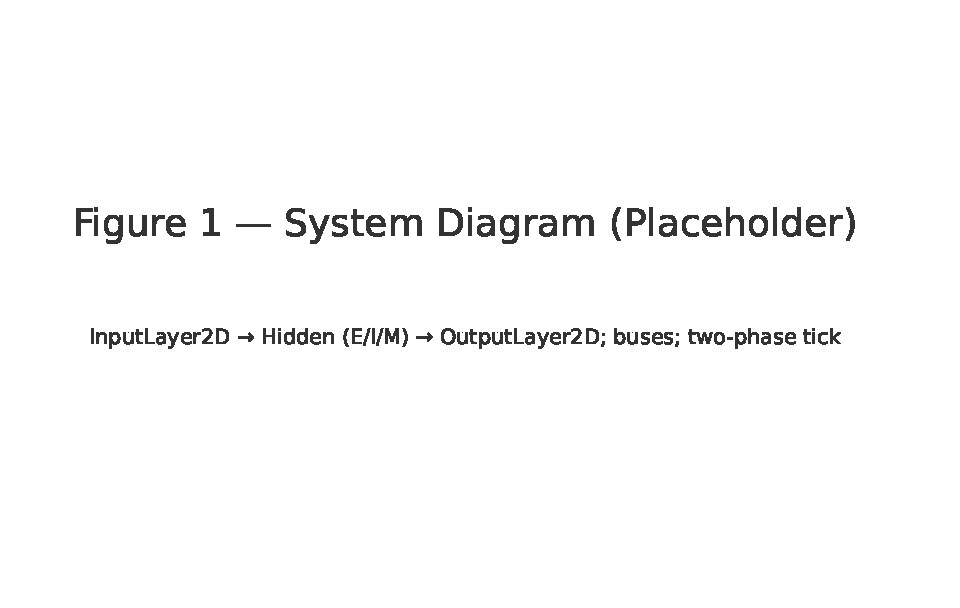
\includegraphics[width=0.95\linewidth]{figures/fig_system.pdf}
  \caption{GrowNet system overview.}
  \label{fig:system}
\end{figure}

\begin{figure}[t]
  \centering
  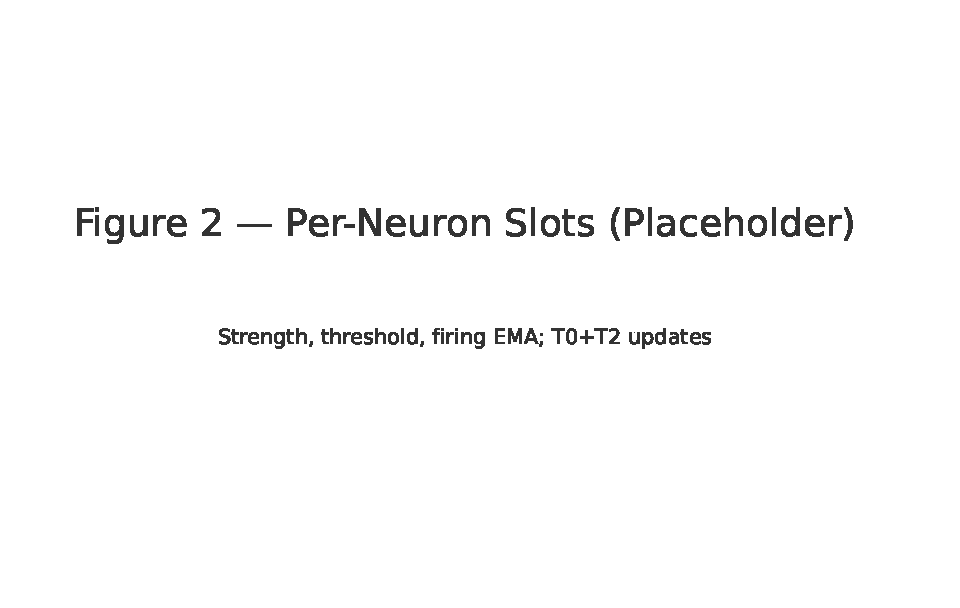
\includegraphics[width=0.85\linewidth]{figures/fig_slot_closeup.pdf}
  \caption{Per-neuron slot close-up with adaptive thresholds (T0+T2).}
  \label{fig:slot}
\end{figure}

\begin{figure}[t]
  \centering
  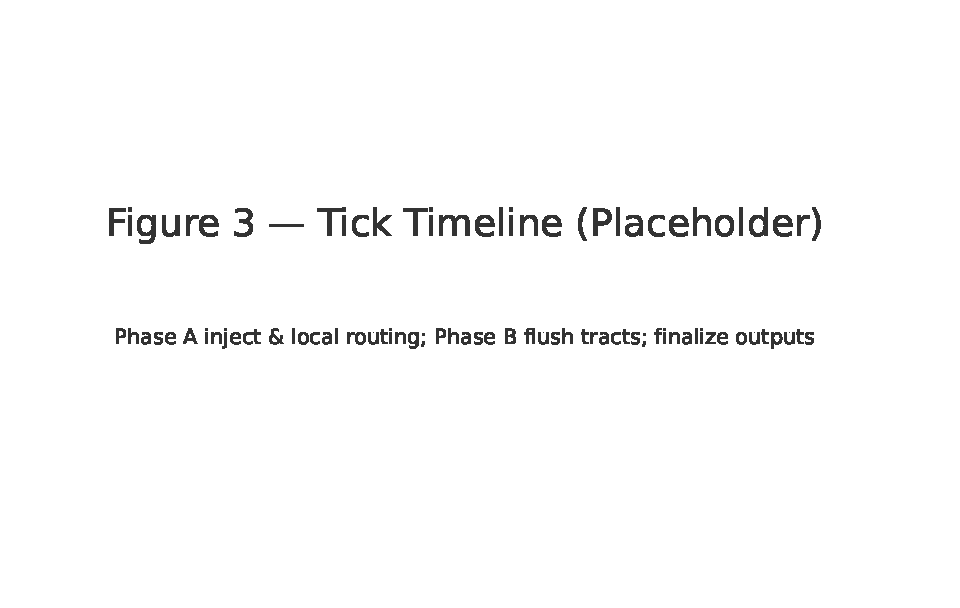
\includegraphics[width=0.95\linewidth]{figures/fig_tick_timeline.pdf}
  \caption{Two-phase tick timeline.}
  \label{fig:timeline}
\end{figure}


\section{Experiments}
\paragraph{Benchmarks.} Few-shot Omniglot-style slices and a simple image moving-dot demo; plus one domain-specific stream.

\paragraph{Metrics.} Accuracy vs.\ examples, delivered events, stability under continual updates, growth events, and compute/runtime.

\paragraph{Ablations.} Remove growth, remove T2, disable bus effects, single-slot only vs.\ multi-slot hidden layers.

\section{Results}
We report sample-efficiency and stability plots, and visualize slot counts over time. Key numbers are summarized in Table~\ref{tab:main}.

\section{Limitations and Broader Impact}
GrowNet is not biologically exact and currently relies on simple wiring and growth triggers. GPU/vectorized kernels are deferred; large-scale tasks remain future work. Ethical considerations include energy usage and potential misuse; we provide code for reproducibility.

\section{Conclusion}
We presented GrowNet, a learning-first, locally updated network with slot-gated neurons and growth-on-demand. Early results suggest strong data efficiency with stable continual learning. Future work includes learned wiring policies and neuromodulator broadcasts across regions.

\bibliographystyle{plainnat}
\bibliography{main}

% The official NeurIPS checklist is included via the style; keep it enabled.
% Follow the NeurIPS CFP and checklist guidance precisely.

\end{document}